\section{Tokenizer Ablation}
\label{sec:ablation}

The main experiment gives every method the same Kiwi morphemes. A natural objection is
that a stronger \emph{TF-IDF} representation---character $n$-grams, which are robust to
spelling variation and need no analyser---might remove the neural advantage. We
therefore re-run, for each dataset, the best TF-IDF and the best neural method (selected by
mean validation macro-F1 at $n=8{,}000$ in the main sweep: \ablationTfidfNSMC{} and
\ablationNeuralNSMC{} on NSMC, \ablationTfidfShopping{} and \ablationNeuralShopping{} on
Shopping, \ablationTfidfSteam{} and \ablationNeuralSteam{} on Steam) with three
tokenizers: eojeol (whitespace) unigrams+bigrams, Kiwi morphemes, and character
2--4-grams for TF-IDF (single characters for neural models), at $n=500$ and $8{,}000$
with all \nSeeds{} seeds (\nAblationFits{} new fits). Vocabulary, TF-IDF and maximum
length (eojeol: \maxSeqLenWhitespace, character: \maxSeqLenChar{} tokens) are rebuilt per
tokenizer; hyperparameters are the frozen, Kiwi-tuned ones.

\begin{table}[t]
  \centering
  \caption{Tokenizer ablation: test macro-F1 ($\times100$) of the best TF-IDF and best
  neural method per dataset with eojeol, Kiwi and character tokenization. \pmnote{}
  Bold: best tokenizer for the method and size (test); $^{\star}$: best tokenizer selected on
  validation. ``Gap, best tok.'': paired neural $-$ TF-IDF gap (points) when each family
  uses its validation-selected best tokenizer, with the main (Kiwi) gap for comparison.}
  \label{tab:ablation}
  % AUTO-GENERATED by ksent.analysis.make_tables (do not edit by hand).
\begin{adjustbox}{max width=\linewidth}
\begin{tabular}{llrrrrrr}
\toprule
Dataset & Method & \multicolumn{3}{c}{$n$=500} & \multicolumn{3}{c}{$n$=8{,}000} \\
\cmidrule(lr){3-5}\cmidrule(lr){6-8}
 & & Eojeol & Kiwi & Char & Eojeol & Kiwi & Char \\
\midrule
\multirow{3}{*}{NSMC} & best TF-IDF & -- & -- & -- & -- & -- & -- \\
 & best neural & -- & -- & -- & -- & -- & -- \\
 & \textit{Gap, best tok.} & \multicolumn{3}{c}{--} & \multicolumn{3}{c}{--} \\
\midrule
\multirow{3}{*}{Shopping} & best TF-IDF & -- & -- & -- & -- & -- & -- \\
 & best neural & -- & -- & -- & -- & -- & -- \\
 & \textit{Gap, best tok.} & \multicolumn{3}{c}{--} & \multicolumn{3}{c}{--} \\
\midrule
\multirow{3}{*}{Steam} & best TF-IDF & -- & -- & -- & -- & -- & -- \\
 & best neural & -- & -- & -- & -- & -- & -- \\
 & \textit{Gap, best tok.} & \multicolumn{3}{c}{--} & \multicolumn{3}{c}{--} \\
\bottomrule
\end{tabular}
\end{adjustbox}

\end{table}

\begin{figure}[t]
  \centering
  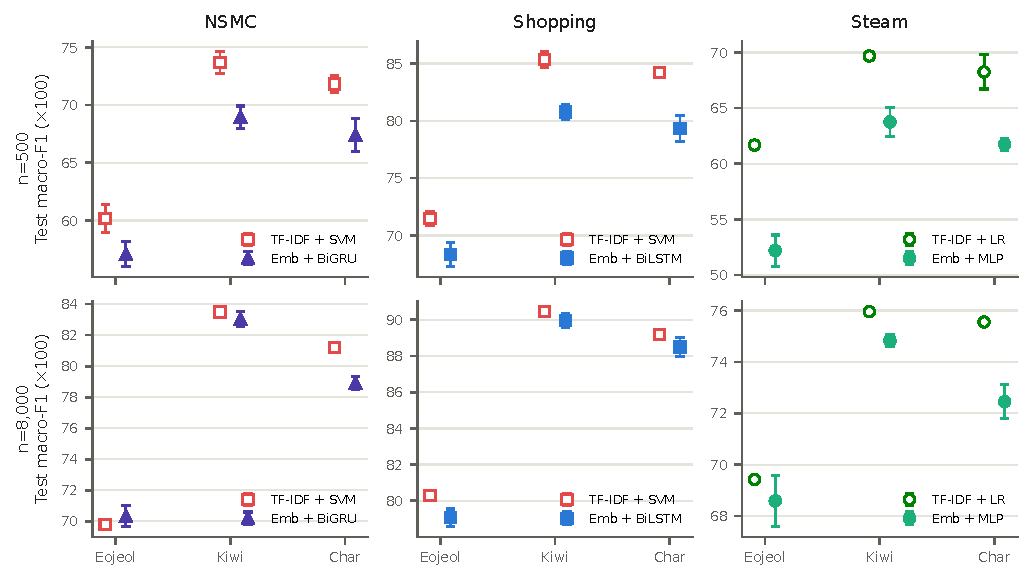
\includegraphics[width=\linewidth]{figures/fig5_tokenizers.pdf}
  \caption{Tokenizer effect: test macro-F1 of the best TF-IDF (hollow) and best neural
  (filled) method per dataset at $n=500$ (top) and $n=8{,}000$ (bottom); error bars are
  $\pm1$ std over \nSeeds{} seeds (sample std).}
  \label{fig:tokenizers}
\end{figure}

With each family using its best tokenizer, the neural $-$ TF-IDF gap is \ablationGapSmallNSMC{}
(NSMC), \ablationGapSmallShopping{} (Shopping) and \ablationGapSmallSteam{} (Steam) points
at $n=500$, and \ablationGapLargeNSMC, \ablationGapLargeShopping{} and
\ablationGapLargeSteam{} points at $n=8{,}000$ (\cref{tab:ablation,fig:tokenizers}). The best
TF-IDF tokenizer at 8{,}000 is \bestTokenizerTfidfNSMC/\bestTokenizerTfidfShopping/\bestTokenizerTfidfSteam{}
and the best neural tokenizer \bestTokenizerNeuralNSMC/\bestTokenizerNeuralShopping/\bestTokenizerNeuralSteam{}
(NSMC/Shopping/Steam). The main conclusion (whether the gap reaches \crossoverMargin{} point)
holds with the best tokenizers on NSMC: \ablationHoldsNSMC; Shopping: \ablationHoldsShopping;
Steam: \ablationHoldsSteam.

A stronger TF-IDF representation does not change the picture, because character $n$-grams
are \emph{not} stronger here. Kiwi morphemes are the best tokenizer for both families in
almost every cell of \cref{tab:ablation}, and eojeol tokens are clearly the worst. Korean
attaches particles and endings to the stem, so whole eojeol are sparse and most of them
are unseen at small sizes. The single exception is Shopping at $n=8{,}000$. There,
validation selects character $n$-grams for TF-IDF, but on test they do worse than Kiwi
morphemes. The paired gap with each family's validation-selected tokenizer therefore turns
positive (\ablationGapLargeShopping{} points). It still stays below the
\crossoverMargin-point margin, and it comes from a selection miss on the TF-IDF side, not
from a neural gain. Kiwi's linguistic knowledge helps both families. Removing it (eojeol or
characters) costs the TF-IDF and the neural model similar amounts, with no consistent
advantage for either. The conclusion of the main experiment (no crossover up to 8{,}000) is therefore not
an artefact of the tokenizer choice.
